\chapter{Introduction}

Le but de ce projet est de développer une plateforme de signalement pour la maintenance des
infrastructures d'une organisation. Cette plateforme permettra aux usagers de signaler une
anomalie sur une ressource simplement en scannant un QR code.

\chapter{Architecture}

\section{Modèle de la base de données}
La première étape de la conception était de décider du modèle de la base de données. Le schéma
suivant décrit le schéma des tables que nous avons choisi :\newline

\begin{figure}[!h]
    \centering
    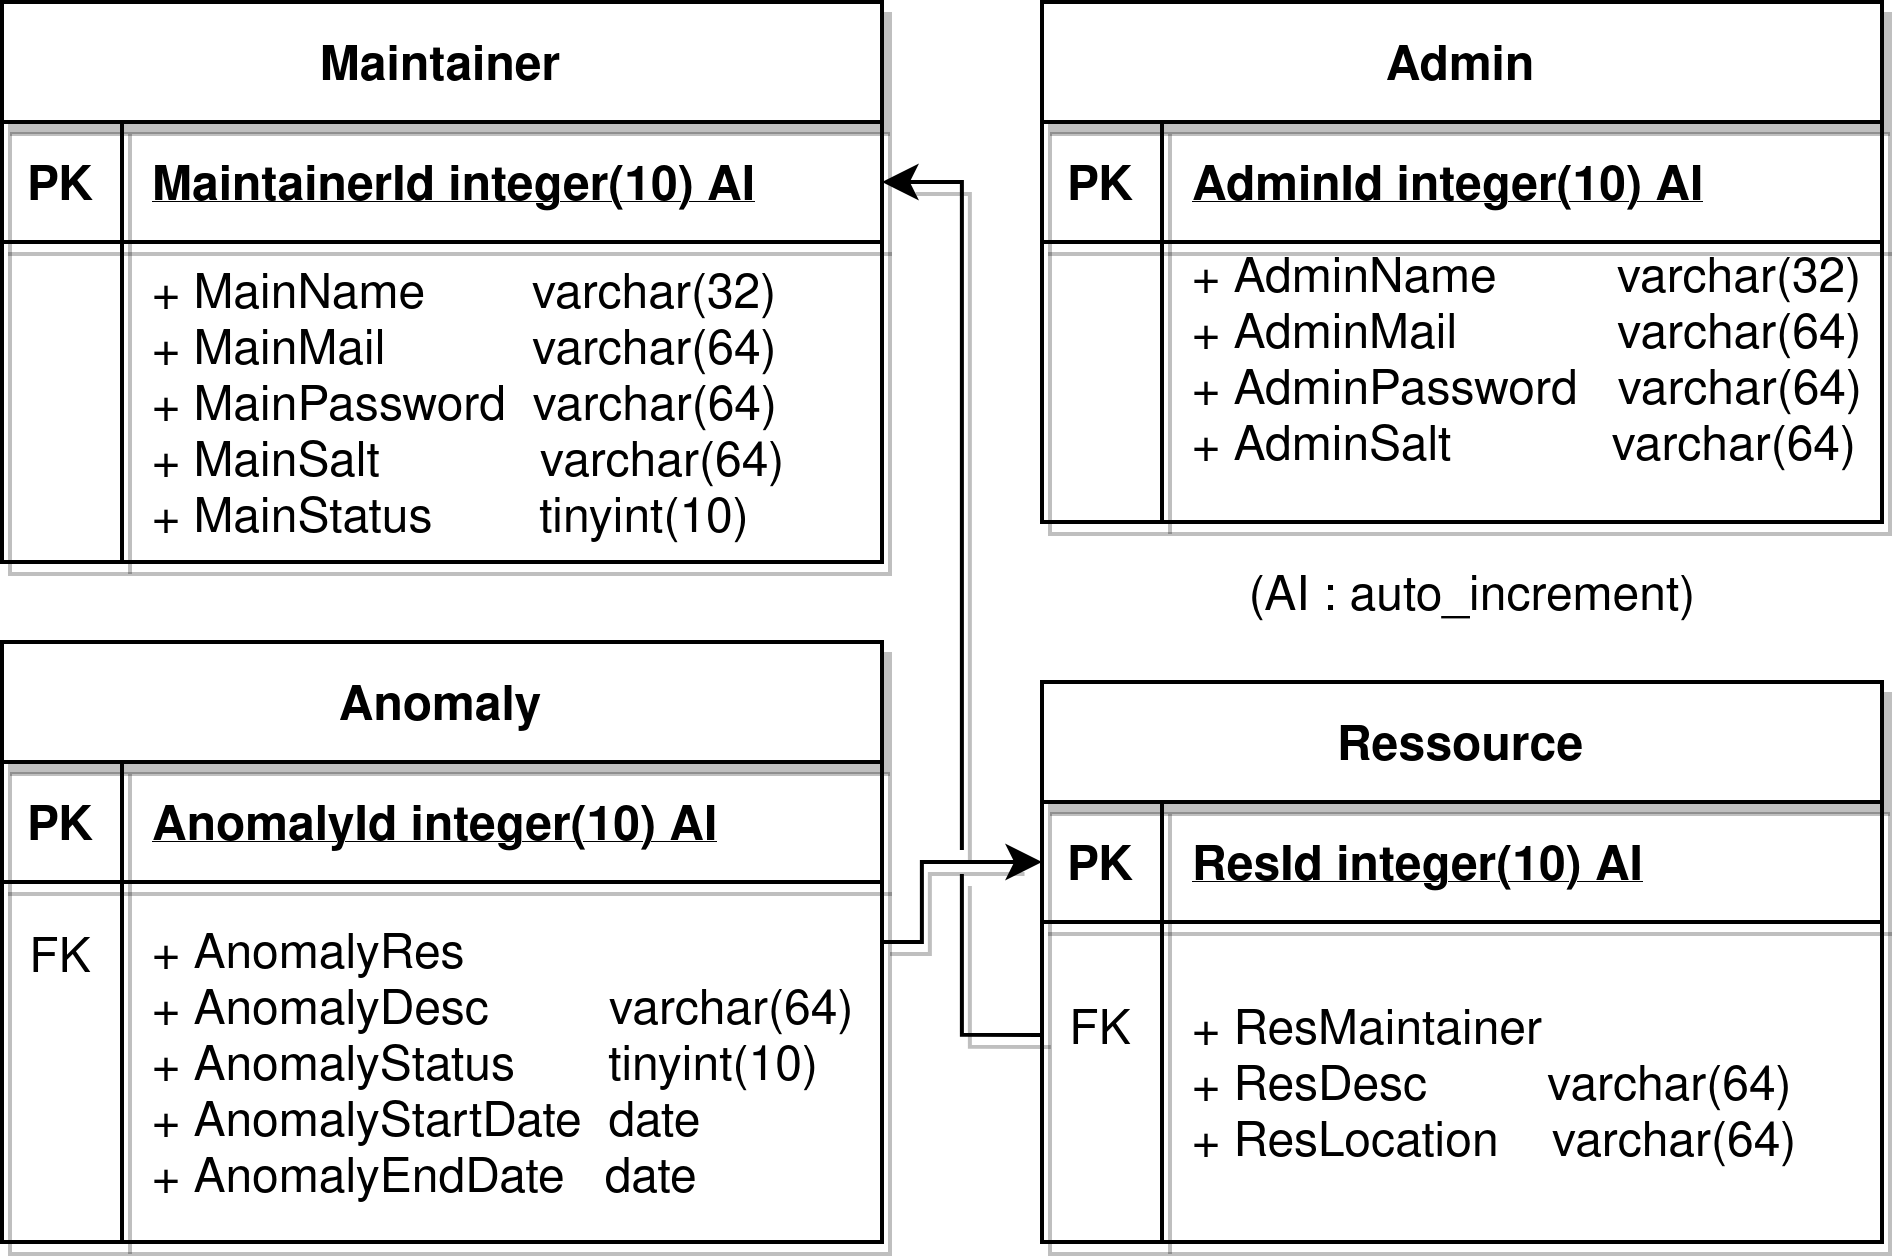
\includegraphics[width=\textwidth]{img/schemaSQL.png}
    \caption{Schéma des tables de la base de données}
    \label{fig:schemaSQL}
\end{figure}
\newpage

\section{Modèle MVC}
L'application a été conçu en suivant le modèle MVC (Modèle-Vue-Contrôleur). C'est le modèle le
plus simple et le plus utilisée.

\section{Technologies choisies}
La partie vue est écrite dans les langages classiques : HTML \& CSS. Nous n'avons pas utiliser
de JavaScript pour la plateforme.\newline

Nous avons choisis d'utiliser Java avec les Servlets et les JSP pour développer la partie
contrôleur de l'application.\newline

Le modèle est donc écrit en Java en utilisant la bibliothèque JDBC pour les interactions avec
le SGBD (MySQL). Nous avons premièrement implémenter des classes Java décrivant simplement le
modèle des types d'objets utilisés, c'est-à-dire :
\begin{itemize}
    \item \verb:User: : classe des utilisateurs,
    \item \verb:Admin: : classe des administrateurs, héritant de \verb:User:,
    \item \verb:Maintainer: : classe des responsables de maintenance, héritant de \verb:User:,
    \item \verb:Ressource: : classe des ressources,
    \item \verb:Anomaly: : classe des anomalies.
\end{itemize}
Ensuite pour chacune des classes exceptées \verb:User: nous avons écrit une classe correspondante
qui fait l'intermédiaire entre le SGBD et le modèle, selon le modèle DAO (Data Access Object).


\subsection{Frameworks}
Pour développer la plateforme nous avons utilisés un framework pour le CSS :
\textbf{Bootstrap}.
Cela nous a permis de simplifier grandement le développement de la vue afin de se concentrer sur
le back-end.

\section{Sécurisation}
Afin de sécuriser au mieux la plateforme nous avons mis en place les sécurités suivantes :
\begin{description}
    \item[\textbf{Filtrage des urls:}] via un filter JEE.
    \item[\textbf{Requête préparées:}] en utilisant la bibliothèque JDBC.
\end{description}

\chapter{Difficultés}

\chapter{Conclusion}

\chapter{Annexe}

\section{Notice d'utilisation}

L'installation peut se faire de deux manières différentes :

\begin{enumerate}
    \item Premièrement, copier l'archive \verb:install.tar.gz: sur la machine cible, ensuite
        l'extraire puis lancer le script \verb:install.sh: avec les droits administrateurs.

    \item Sinon l'application peut être installer directement depuis la machine cible en recupérant
        le script d'installation sur GitHub et en lançant le script comme precédemment :
\end{enumerate}

\begin{minted}{bash}
wget https://raw.githubusercontent.com/loukabvn/projet-web/main/install.sh
chmod u+x install.sh
su root
./install.sh
\end{minted}

Il faut ensuite renseigner les informations demandées c'est-à-dire les identifiants pour le
compte MySQL pour l'accès administrateur à la base de données et les identifiants pour le compte
administrateur de la plateforme.

Une fois l'installation terminée vous pouvez vous rendre sur :
\begin{center}
    \url{http://192.168.76.76:8080/ProjetWeb/home}
\end{center}
et vous connecter avec les identifiants renseignés.

\section{Jeu de données}

Un jeu de données pré-rempli est disponible pour effectuer des tests sur notre plateforme.
Pour pouvoir utiliser ces données il suffit d'exécuter avec mysql le script \verb:insertion.sql:.
Également, durant l'installation, l'insertion de ce jeu de données de test vous ait proposé, que
vous pouvez accepter ou refuser.

